\documentclass{beamer}
\usepackage{amsmath}
\usepackage{xcolor}

\usetheme{default}
\usecolortheme{beaver}
\usefonttheme[onlymath]{serif}

\title{Utilizing reinforcement learning techniques to play Atari's Breakout}
\author{Andrew~Messing \and Ben~Brock \and Cory~Walker}
\date{November 24, 2015}
\subject{Computer Science}

\AtBeginSection[]
{
  \begin{frame}<beamer>{Outline}
    \tableofcontents[currentsection,currentsubsection]
  \end{frame}
}

\DeclareMathOperator*{\argmin}{arg\,min}
\DeclareMathOperator*{\argmax}{arg\,max}

\begin{document}

\begin{frame}
  \titlepage
\end{frame}

\begin{frame}{Outline}
  \tableofcontents
\end{frame}

% Section and subsections will appear in the presentation overview
% and table of contents.
\section{Feature extraction}

\begin{frame}{First Slide Title}
  \begin{itemize}
  \item {
    My first point.
  }
  \item {
    My second point.
  }
  \end{itemize}
\end{frame}

\begin{frame}{First Slide Title}
  \begin{itemize}
  \item {
    My first point.
  }
  \item {
    My second point.
  }
  \end{itemize}
\end{frame}

\section{Reinforcement learning}

\begin{frame}{Blocks}
\begin{block}{Block Title}
You can also highlight sections of your presentation in a block, with it's own title
\end{block}
\begin{theorem}
There are separate environments for theorems, examples, definitions and proofs.
\end{theorem}
\begin{example}
Here is an example of an example block.
\end{example}
\end{frame}

\section{Deep reinforcement learning}

\begin{frame}{Problem definition}
  \begin{itemize}
  \item {
    Learn Atari games from raw pixels
  }
  \item {
    Google DeepMind
  }
  \item {
      Naive state space: $128^{210 \cdot 160} \approx 1.799\times 10^{70802}$
  }
  \item {
      Grayscale state space: $4^{210 \cdot 160} \approx 1.643\times 10^{20229}$
  }
  \item {
      Scaled grayscale state space: $4^{105 \cdot 80} \approx 2.013\times 10^{5057}$
  }
  \item {
    Still too huge
  }
  \item {
    And partially observable
  }
  \item {
    Generalization is essential
  }
  \end{itemize}
\end{frame}

\begin{frame}{Deep Q network}
  \begin{figure}[H]
    \centering
    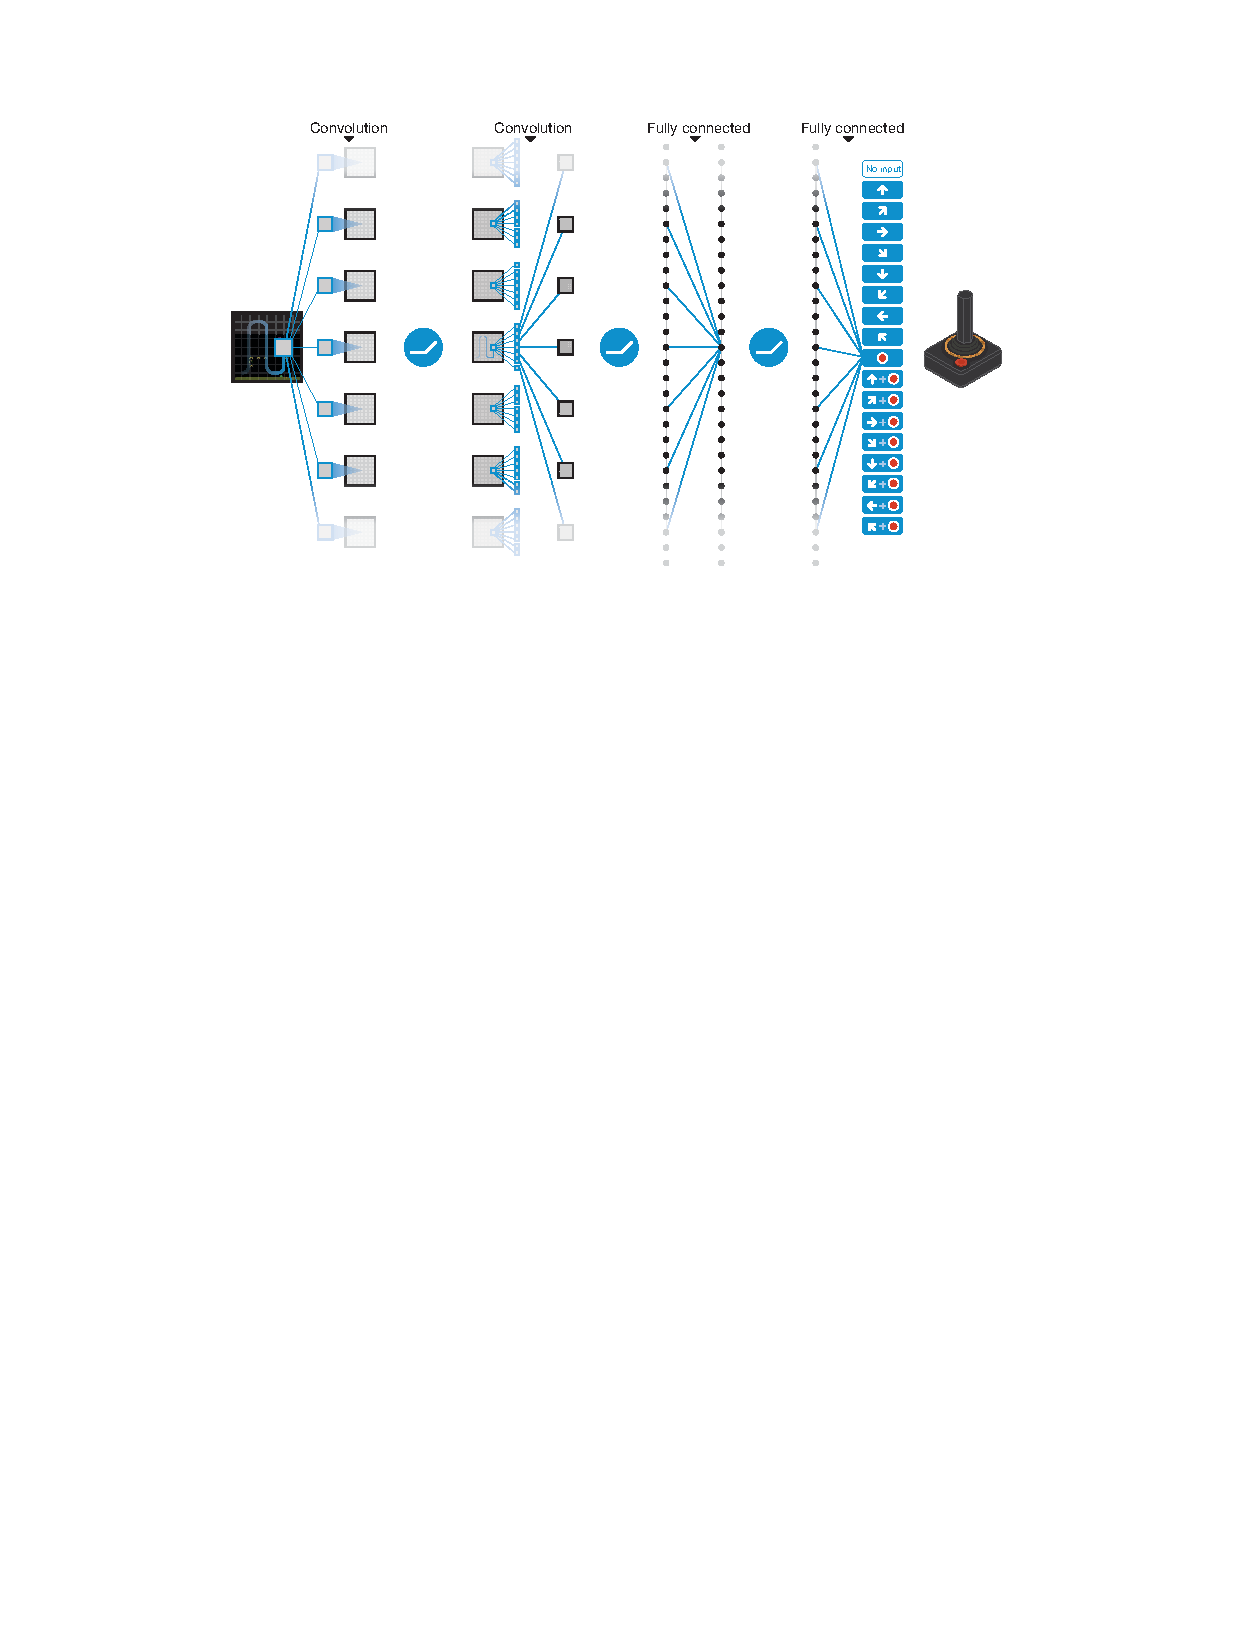
\includegraphics[width=105mm]{deep_q_network.pdf}
  \end{figure}
  \[ \boldsymbol{\theta}_{t+1} = \boldsymbol{\theta}_t+\alpha(Y_t^Q-Q(S_t,A_t;\boldsymbol{\theta}_t))\nabla_{\boldsymbol{\theta}_t}Q(S_t,A_t;\boldsymbol{\theta}_t) \]
\end{frame}

\begin{frame}{DQN variations}
  \begin{itemize}
  \item {
      NIPS (late 2013) - original paper from workshop, 24 hour training time
  }
  \item {
      Nature (early 2015) - similar to NIPS, more conservative hyperparameters (7 day training), model freezing
  }
  \item {
      Double DQN (September 2015) - branch from Nature model, attempts to address value overestimates
  }
  \end{itemize}
\end{frame}

\begin{frame}{Double DQN formulation}
  \begin{itemize}
    \item max operator means we use same values for action selection and evaluation, want to decouple.
    \item Action-value function has weights $\boldsymbol{\theta}_t$
    \item Target action-value function has weights $\boldsymbol{\theta}_t^-$
    \item After every 10,000 training updates, $\boldsymbol{\theta}_t^- \leftarrow \boldsymbol{\theta}_t$
  \end{itemize}

  \[Y_t^{\textrm{DQN}} \equiv R_{t+1} + \gamma \textcolor{red}{\max_{a} Q(S_{t+1},a;\boldsymbol{\theta}_t^-)} \]
  \[ \Downarrow \]
  \[\boxed{Y_t^{\textrm{DoubleDQN}} \equiv R_{t+1} + \gamma \textcolor{red}{Q(S_{t+1},\argmax_a Q(S_{t+1},a;\boldsymbol{\theta}_t),\boldsymbol{\theta}_t^-)}} \]
  \begin{itemize}
    \item If $\boldsymbol{\theta}_t^- = \boldsymbol{\theta}_t$ (NIPS model), no difference
  \end{itemize}
\end{frame}

\begin{frame}{Implementation}
  \begin{itemize}
    \item Nathan Sprague, \href{https://github.com/spragunr/deep_q_rl}{https://github.com/spragunr/deep\_q\_rl}
    \item Circular buffer for 1M replay frames, visualization code, model saving and loading
    \item Already supported NIPS and Nature algorithms.
    \item After some Theano debugging, my fork now supports Double DQN
    \item EC2 g2.2xlarge
    \item Single threaded, CPU bound, 30\% GPU utilization, 8GB replay buffer
  \end{itemize}
\end{frame}

\begin{frame}{Double DQN Results}
  \begin{figure}[H]
    \centering
    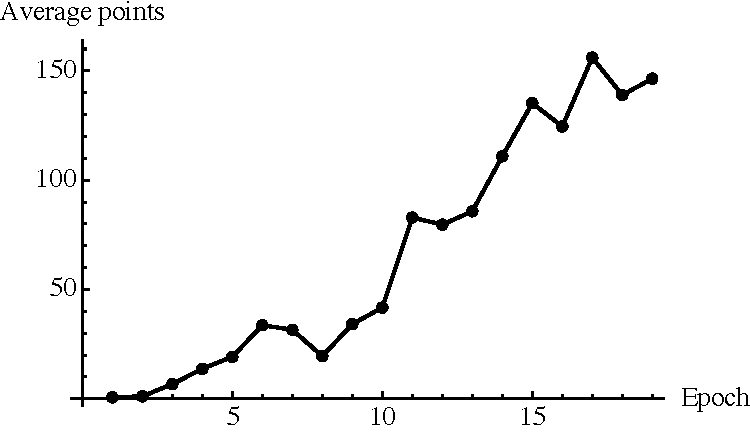
\includegraphics[width=90mm]{dqn_rewardper.pdf}
  \end{figure}
  Each epoch takes about an hour. Stopped after $\sim 20$ hours.
\end{frame}

\begin{frame}{Double DQN Results}
  \begin{figure}[H]
    \centering
    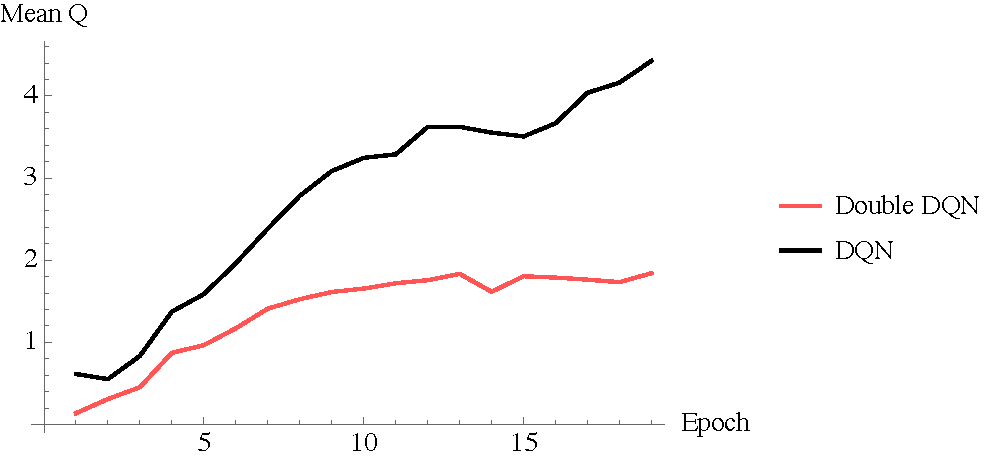
\includegraphics[width=90mm]{dqn_meanq.pdf}
  \end{figure}
\end{frame}


% Placing a * after \section means it will not show in the
% outline or table of contents.
\section*{Summary}

\begin{frame}{Summary}
  \begin{itemize}
  \item
    The \alert{first main message} of your talk in one or two lines.
  \item
    The \alert{second main message} of your talk in one or two lines.
  \item
    Perhaps a \alert{third message}, but not more than that.
  \end{itemize}
  
  \begin{itemize}
  \item
    Outlook
    \begin{itemize}
    \item
      Something you haven't solved.
    \item
      Something else you haven't solved.
    \end{itemize}
  \end{itemize}
\end{frame}



% All of the following is optional and typically not needed. 
\appendix
\section<presentation>*{\appendixname}
\subsection<presentation>*{For Further Reading}

\begin{frame}[allowframebreaks]
  \frametitle<presentation>{For Further Reading}

  \begin{thebibliography}{10}

  \beamertemplatebookbibitems

  \bibitem{suttonbarto}
    Sutton, R. S., \& Barto, A. G. (1998). \textit{Reinforcement learning: An introduction} (Vol. 1, No. 1). Cambridge: MIT press.

  \beamertemplatearticlebibitems

  \bibitem{dmnips}
    Mnih, V., Kavukcuoglu, K., Silver, D., Graves, A., Antonoglou, I., Wierstra, D., \& Riedmiller, M. (2013). Playing Atari with deep reinforcement learning. \textit{arXiv preprint arXiv:1312.5602}.

  \bibitem{dmdoubl}
    van Hasselt, H., Guez, A., \& Silver, D. (2015). Deep Reinforcement Learning with Double Q-learning. \textit{arXiv preprint arXiv:1509.06461}.
  \end{thebibliography}
\end{frame}

\end{document}
